\chapter{User Manual}

This appendix explains the project operation by running the ``Scenario 1:
Emergencies-Lorca Earthquake'' defined in appendix~\ref{anex:scenarios}. To do
this the experimenters must first create an account in \emph{Fed4FIRE} platform
and after that, they can already run the experiment. Then, the \emph{Rspec} of the nodes in
\vw is obtained from \emph{JFed} and using it, the \ac{GUI} provides an
automatic way to carry out the scenario.

\section{First steps}

For experimenting with Fed4FIRE testbeds, the following steps have to be
done (for more information, see \url{http://doc.fed4fire.eu/}): 
\begin{itemize}
\item To create an account in Fed4FIRE in order to get some certificates
  to access testbeds.
\item To create an account in \bonfire for getting access in this testbed. At
  this moment, in order to use BonFIRE, the experimenters also need to register for an additional account. 
\item To create a \ac{SSH} key and upload in both the \emph{Emulab} and the
  \bonfire account.
\item To download the X.509 certificate which authorizes and authenticates
  experimenters on testbeds.
\end{itemize}

\subsection{Creating a Fed4FIRE account}

The Fed4FIRE webpage for creating an account is available in
\url{http://www.wall2.ilabt.iminds.be}. Once the page was loaded, the user has
to select the option ``Request an Account'' which is located on the middle of the page.

\begin{figure}[!h]
\begin{center}
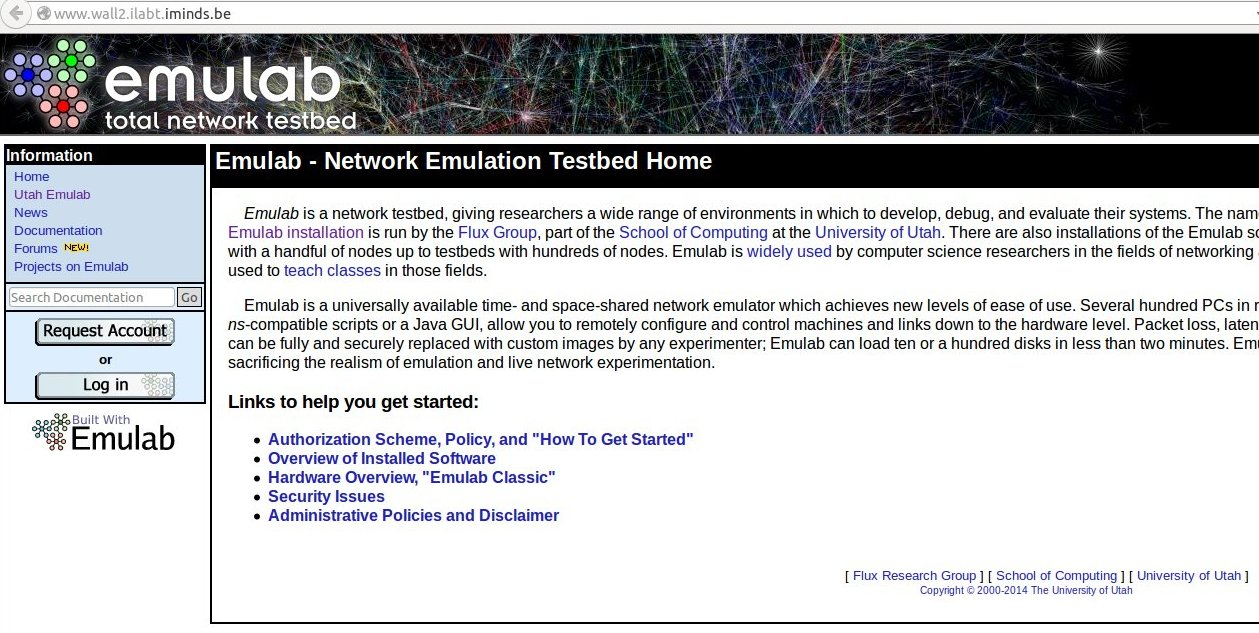
\includegraphics[width=0.7\textwidth]{user-manual/emulab.jpg}
\caption{Fed4FIRE webpage for creating an account}
\label{fig:fed4fire-account}
\end{center}
\end{figure}

Then, the experimenter must fill the registration form and to click in ``Submit''
button. The account is created and it shall be validated by the \emph{Fed4FIRE}
reviewers. 

\subsection{Creating a BonFIRE account}

For obtaining a BonFIRE account, the experimenter has to visit the platform webpage
\url{http://portal.bonfire-project.eu/}. Then, the experimenter fills the
registration form and sends it for approving. 

\begin{figure}[!h]
\begin{center}
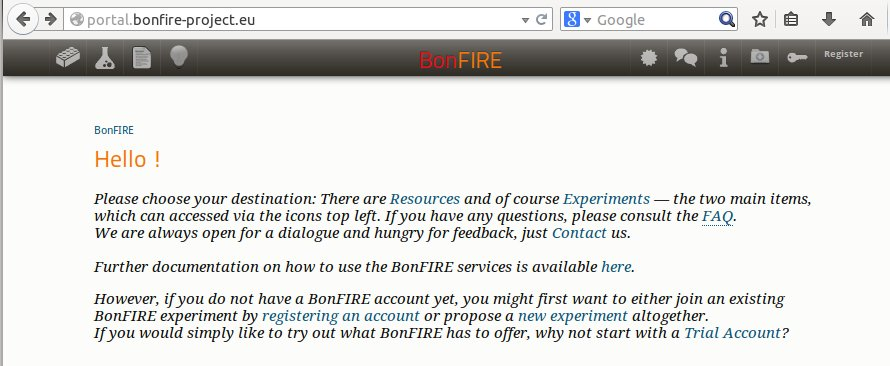
\includegraphics[width=0.7\textwidth]{user-manual/bf.jpg}
\caption{BonFIRE platform webpage}
\label{fig:bonfire-account}
\end{center}
\end{figure}

\subsection{Creating a SSH key}

Once the experimenter registered in the \emph{Fed4FIRE} platforms, it is
necessary to create a pair of \ac{RSA} keys and to upload the generated public key to
\bonfire and \emph{Fed4FIRE} web plattforms. The creation of the \ac{RSA} keys,
depending on the operative system, can be done as follows:
\begin{itemize}
\item \emph{Windows platfomrs}: Using \emph{Putty}. \emph{PuTTY} is a widely
  used \ac{SSH} client for Windows and it includes the tool PuTTYgen to create
  an SSH key. You can download PuTTY from
  \url{http://www.chiark.greenend.org.uk/~sgtatham/putty/download.html}.

\item \emph{Unix platforms}: For UNIX platforms, creating an \ac{SSH} key can be
  done through a command line tool that you run in a terminal. The command that
  performs that is the following: \emph{``ssh-keygen -t rsa''}.

\end{itemize}


\section{Execution of a Scenario}

Once the cloud architecture  and the \sss are running respectively in \bonfire
and \vw and their setups were done \ref{tobedone}, the system is ready for executing the defined scenarios in
annex~\ref{anex:scenarios}. The scenario selected in order to explain this
section was  the ``Scenario 1: Emergencies-Lorca Earthquake''.

Firstly it is necesary to obtain the \emph{Rspec} of the deployed nodes in
\emph{JFed}. Openning \emph{JFed}, the specification is located in ``Rspec
Editor'' tab.

\begin{figure}[!h]
\begin{center}
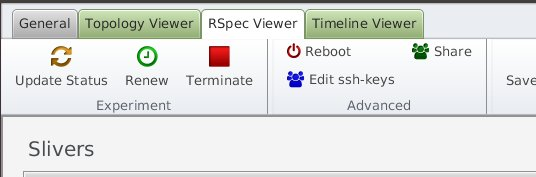
\includegraphics[width=0.7\textwidth]{user-manual/rspec-viewer.jpg}
\caption{Rspec Editor tab in JFed}
\label{fig:rspec-viewer}
\end{center}
\end{figure}


\begin{figure}[!h]
\begin{center}
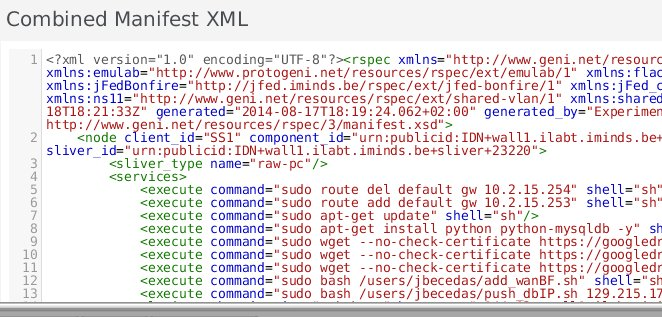
\includegraphics[width=0.7\textwidth]{user-manual/rspec.jpg}
\caption{Rspec in JFed}
\label{fig:rspec}
\end{center}
\end{figure}

The Figure~\ref{fig:rspec} shows the \emph{Rspec} specification which the user
has to fully select and copied into the ``gui/resources/jfed.out'' file,
replacing its content.

Now, the GeoCloud \ac{GUI} can be executed as ``python main.py'' in the
directory of the \emph{GUI}.
The main window appears and the experimenter can select the required scenario.
\begin{figure}[!h]
\begin{center}
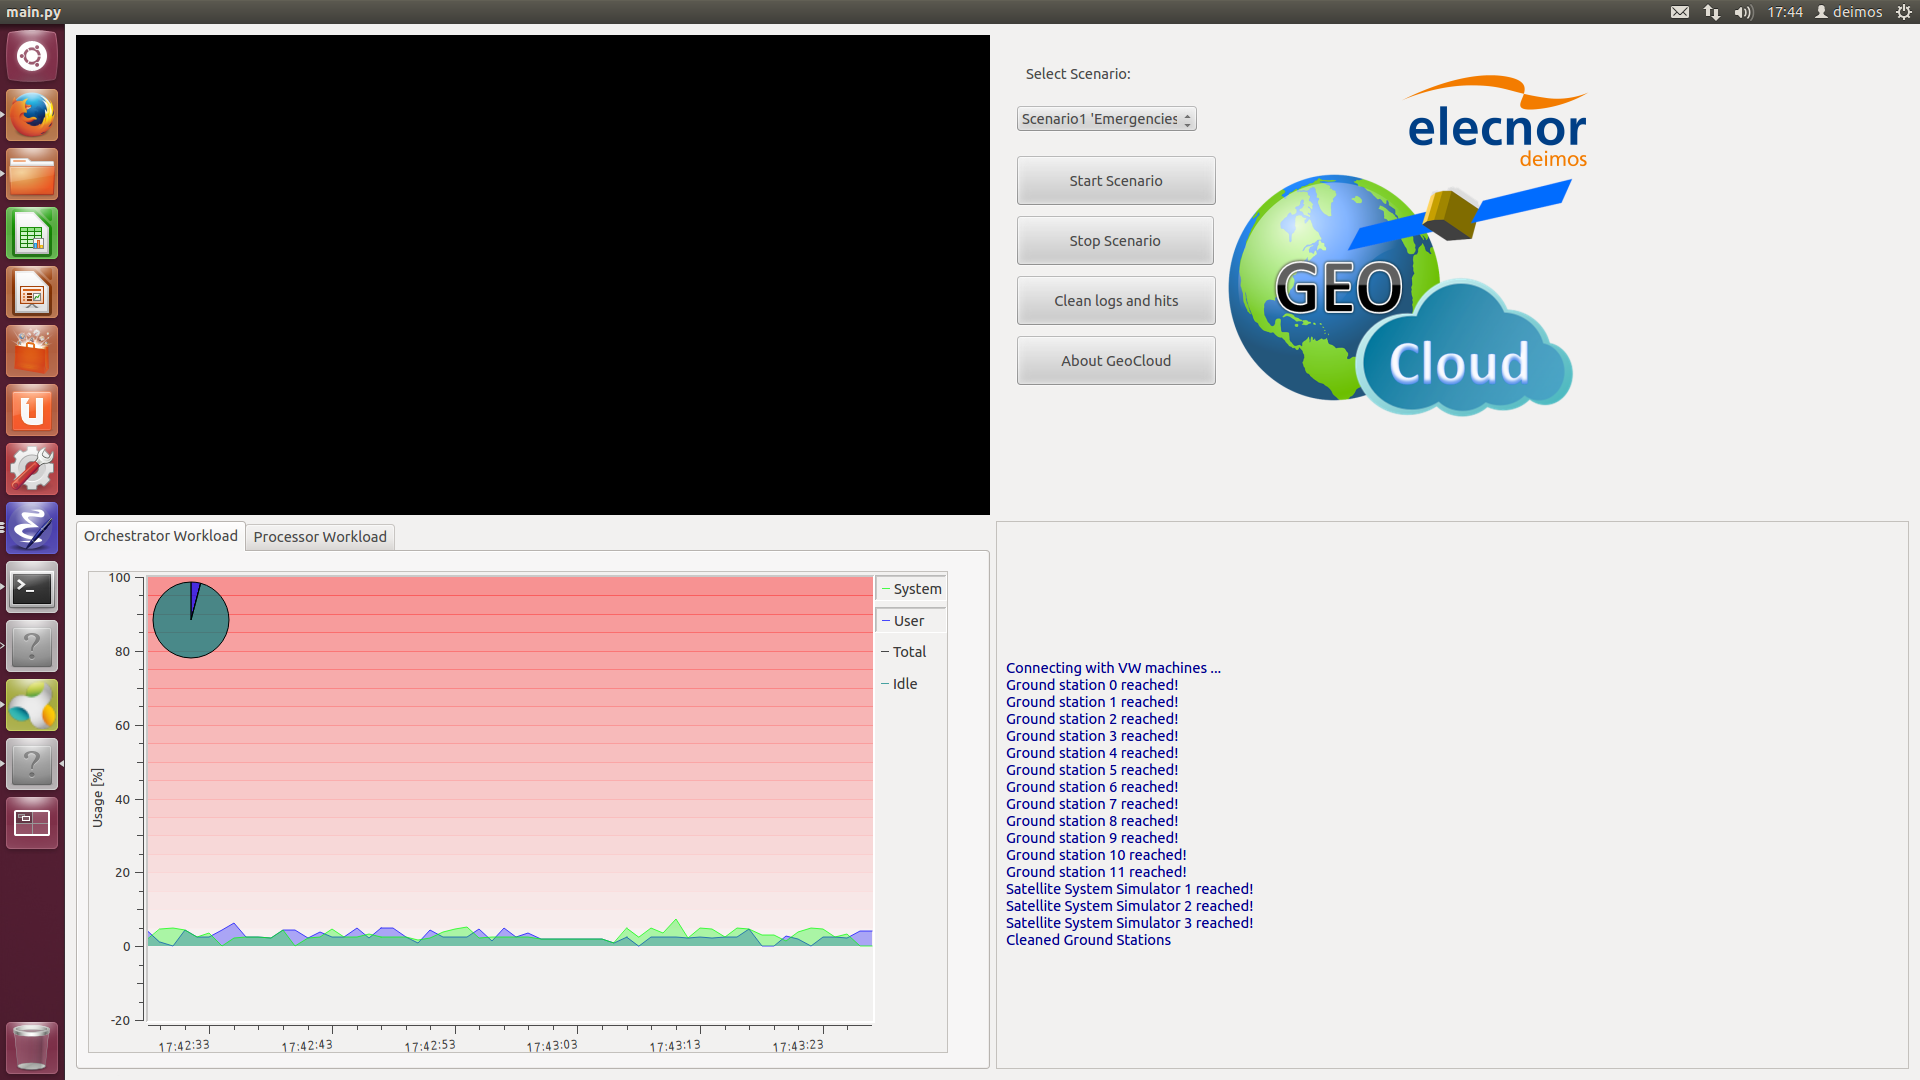
\includegraphics[width=1\textwidth]{user-manual/gui.jpg}
\caption{GUI main window}
\label{fig:gui}
\end{center}
\end{figure}

When the experimenter pushes the start button, the scenario begins to run and
the following actions are carried out: in the Log framework, several messages indicating the state of the execution
appear; in the Workload framework, it is displayed the workload of both orchestrator and
processing chain machines; and in the Video framework, the simulation of the
satellite constelation is displayed.

During the scenario execution, the acquired images from satellites are processed
in the processing chain machine and send to catalogue. In the end, these images are available
in the web service provided by the \emph{Archive and Catalogue} module of the
cloud. 
<<TOBEDONE>>
\begin{figure}[!h]
\begin{center}
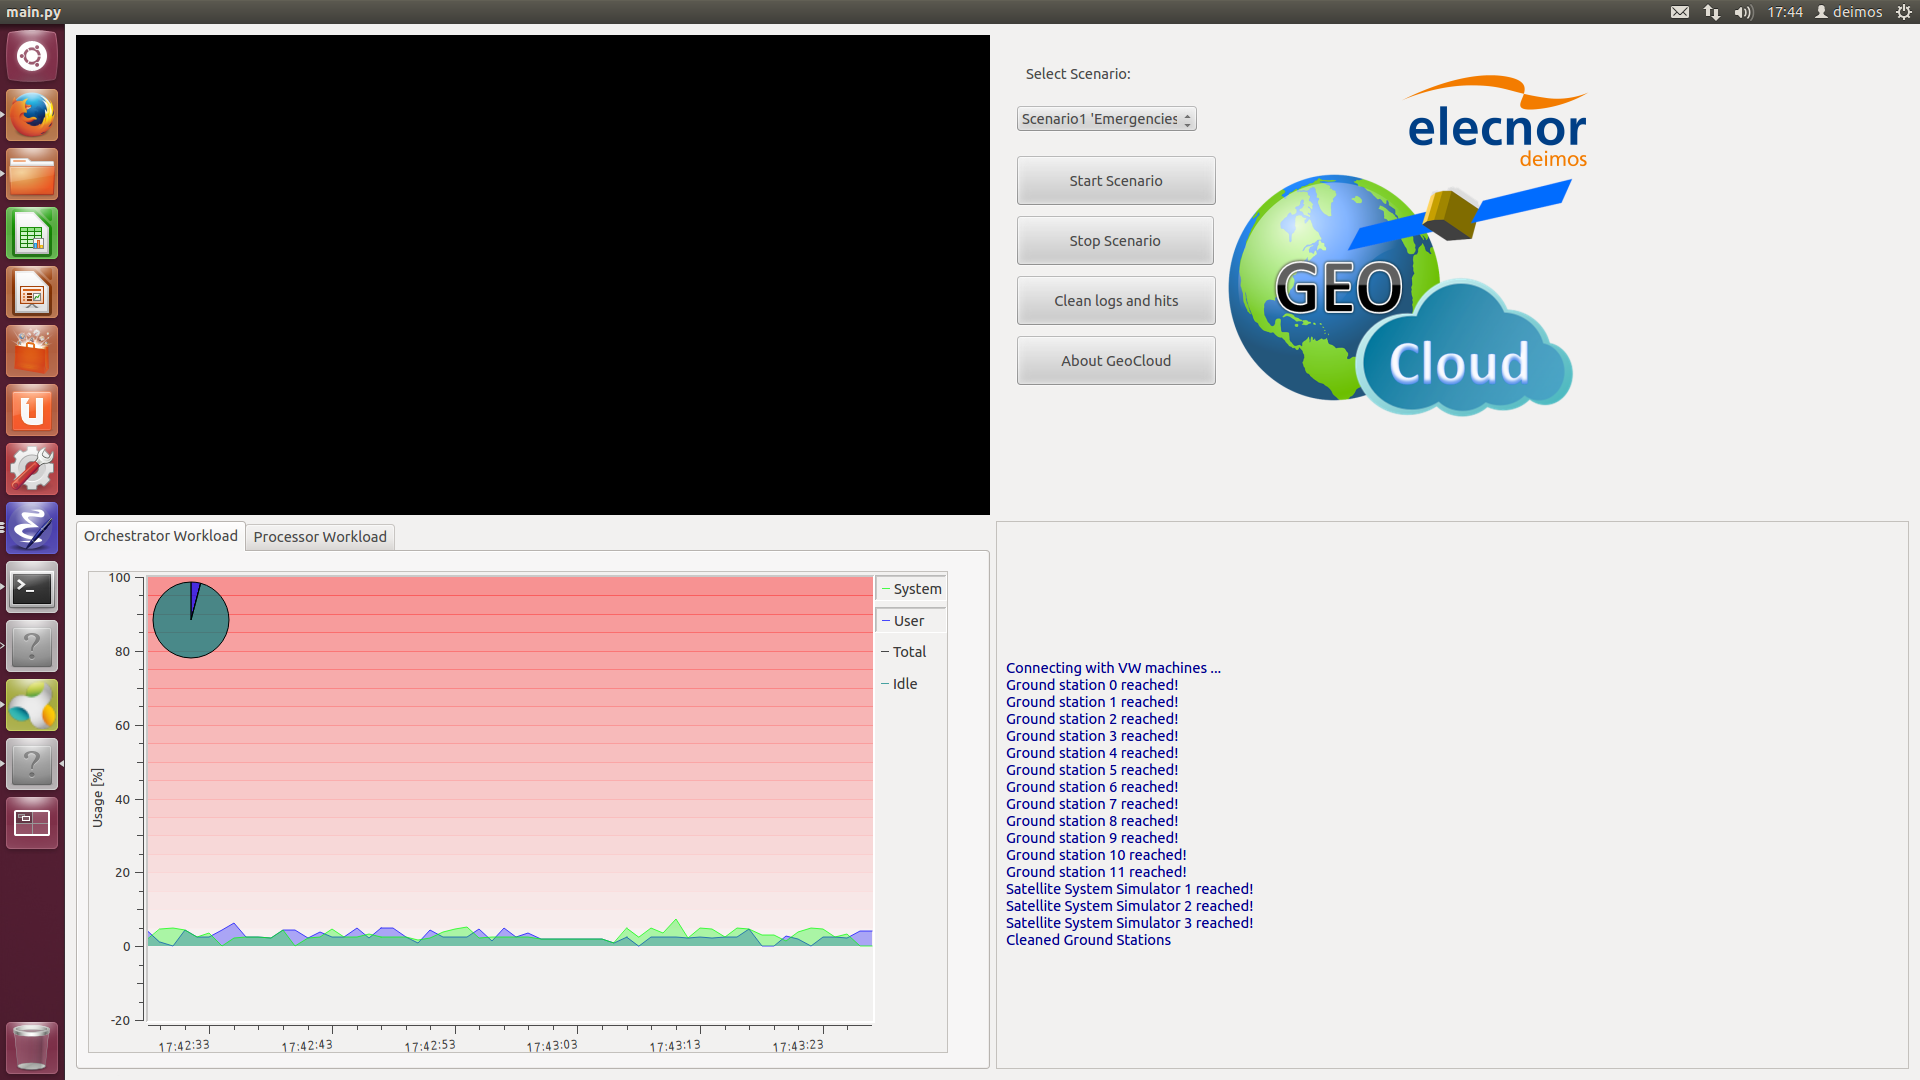
\includegraphics[width=0.7\textwidth]{user-manual/gui.jpg}
\caption{GUI main window}
\label{fig:images-catalogued}
\end{center}
\end{figure}
